% Options for packages loaded elsewhere
\PassOptionsToPackage{unicode}{hyperref}
\PassOptionsToPackage{hyphens}{url}
\PassOptionsToPackage{dvipsnames,svgnames,x11names}{xcolor}
%
\documentclass[
  letterpaper,
  DIV=11,
  numbers=noendperiod]{scrartcl}

\usepackage{amsmath,amssymb}
\usepackage{iftex}
\ifPDFTeX
  \usepackage[T1]{fontenc}
  \usepackage[utf8]{inputenc}
  \usepackage{textcomp} % provide euro and other symbols
\else % if luatex or xetex
  \usepackage{unicode-math}
  \defaultfontfeatures{Scale=MatchLowercase}
  \defaultfontfeatures[\rmfamily]{Ligatures=TeX,Scale=1}
\fi
\usepackage{lmodern}
\ifPDFTeX\else  
    % xetex/luatex font selection
\fi
% Use upquote if available, for straight quotes in verbatim environments
\IfFileExists{upquote.sty}{\usepackage{upquote}}{}
\IfFileExists{microtype.sty}{% use microtype if available
  \usepackage[]{microtype}
  \UseMicrotypeSet[protrusion]{basicmath} % disable protrusion for tt fonts
}{}
\makeatletter
\@ifundefined{KOMAClassName}{% if non-KOMA class
  \IfFileExists{parskip.sty}{%
    \usepackage{parskip}
  }{% else
    \setlength{\parindent}{0pt}
    \setlength{\parskip}{6pt plus 2pt minus 1pt}}
}{% if KOMA class
  \KOMAoptions{parskip=half}}
\makeatother
\usepackage{xcolor}
\setlength{\emergencystretch}{3em} % prevent overfull lines
\setcounter{secnumdepth}{-\maxdimen} % remove section numbering
% Make \paragraph and \subparagraph free-standing
\ifx\paragraph\undefined\else
  \let\oldparagraph\paragraph
  \renewcommand{\paragraph}[1]{\oldparagraph{#1}\mbox{}}
\fi
\ifx\subparagraph\undefined\else
  \let\oldsubparagraph\subparagraph
  \renewcommand{\subparagraph}[1]{\oldsubparagraph{#1}\mbox{}}
\fi


\providecommand{\tightlist}{%
  \setlength{\itemsep}{0pt}\setlength{\parskip}{0pt}}\usepackage{longtable,booktabs,array}
\usepackage{calc} % for calculating minipage widths
% Correct order of tables after \paragraph or \subparagraph
\usepackage{etoolbox}
\makeatletter
\patchcmd\longtable{\par}{\if@noskipsec\mbox{}\fi\par}{}{}
\makeatother
% Allow footnotes in longtable head/foot
\IfFileExists{footnotehyper.sty}{\usepackage{footnotehyper}}{\usepackage{footnote}}
\makesavenoteenv{longtable}
\usepackage{graphicx}
\makeatletter
\def\maxwidth{\ifdim\Gin@nat@width>\linewidth\linewidth\else\Gin@nat@width\fi}
\def\maxheight{\ifdim\Gin@nat@height>\textheight\textheight\else\Gin@nat@height\fi}
\makeatother
% Scale images if necessary, so that they will not overflow the page
% margins by default, and it is still possible to overwrite the defaults
% using explicit options in \includegraphics[width, height, ...]{}
\setkeys{Gin}{width=\maxwidth,height=\maxheight,keepaspectratio}
% Set default figure placement to htbp
\makeatletter
\def\fps@figure{htbp}
\makeatother

\KOMAoption{captions}{tableheading}
\makeatletter
\@ifpackageloaded{caption}{}{\usepackage{caption}}
\AtBeginDocument{%
\ifdefined\contentsname
  \renewcommand*\contentsname{Table of contents}
\else
  \newcommand\contentsname{Table of contents}
\fi
\ifdefined\listfigurename
  \renewcommand*\listfigurename{List of Figures}
\else
  \newcommand\listfigurename{List of Figures}
\fi
\ifdefined\listtablename
  \renewcommand*\listtablename{List of Tables}
\else
  \newcommand\listtablename{List of Tables}
\fi
\ifdefined\figurename
  \renewcommand*\figurename{Figure}
\else
  \newcommand\figurename{Figure}
\fi
\ifdefined\tablename
  \renewcommand*\tablename{Table}
\else
  \newcommand\tablename{Table}
\fi
}
\@ifpackageloaded{float}{}{\usepackage{float}}
\floatstyle{ruled}
\@ifundefined{c@chapter}{\newfloat{codelisting}{h}{lop}}{\newfloat{codelisting}{h}{lop}[chapter]}
\floatname{codelisting}{Listing}
\newcommand*\listoflistings{\listof{codelisting}{List of Listings}}
\makeatother
\makeatletter
\makeatother
\makeatletter
\@ifpackageloaded{caption}{}{\usepackage{caption}}
\@ifpackageloaded{subcaption}{}{\usepackage{subcaption}}
\makeatother
\ifLuaTeX
  \usepackage{selnolig}  % disable illegal ligatures
\fi
\usepackage{bookmark}

\IfFileExists{xurl.sty}{\usepackage{xurl}}{} % add URL line breaks if available
\urlstyle{same} % disable monospaced font for URLs
\hypersetup{
  pdftitle={Assessing the Influence of Pesticide Usage, Parasitic Factors, and Climate on Honey Bee Populations in the United States (2015-2019)},
  pdfauthor={Hanxi Chen, Tianyu Duan, Hanlin Zhao},
  colorlinks=true,
  linkcolor={blue},
  filecolor={Maroon},
  citecolor={Blue},
  urlcolor={Blue},
  pdfcreator={LaTeX via pandoc}}

\title{Assessing the Influence of Pesticide Usage, Parasitic Factors,
and Climate on Honey Bee Populations in the United States (2015-2019)}
\author{Hanxi Chen, Tianyu Duan, Hanlin Zhao}
\date{}

\begin{document}
\maketitle

\renewcommand*\contentsname{Table of contents}
{
\hypersetup{linkcolor=}
\setcounter{tocdepth}{2}
\tableofcontents
}
\section{Introduction}\label{introduction}

\subsection{Project Summary}\label{project-summary}

Flowering plants play vital roles in natural and agricultural
ecosystems, providing food, fiber, and shelter for wildlife and humans
(Calderone, 2012). Pollination, a crucial step in their reproductive
process, is typically necessary for seed production and is primarily
carried out by animals, particularly bees (Calderone, 2012). With
approximately 17,000 described species worldwide, bees are the most
common pollinators (Calderone, 2012). However, the decline in honey bee
colonies and other pollinators raises concerns about the impact on
ecosystems (Calderone, 2012). Therefore, understanding this relationship
is crucial for promoting sustainable agricultural practices and
preserving biodiversity. Our project delves into the intricate
associations between fluctuating levels of pesticide usage, diverse
climate conditions, and the overall health (reflected by percentage
loss) of honey bee populations in the USA.

Through rigorous investigation, we aim to uncover the complex interplay
between these factors, shedding light on their combined effects on honey
bee colonies across the United States. Our ultimate goal is to gain
insights to enhance sustainable agricultural practices and preserve
biodiversity.

In the planned data analysis, the primary focus is on investigating the
interrelationships among pesticide usage, honey bee health metrics, and
climate variables in the dataset spanning from 2015 to 2019. The
analysis will involve correlation studies to uncover potential
associations between these factors, utilizing statistical models to
quantify the strength and direction of relationships after checking
necessary assumptions. This approach is considered optimal for
understanding the intricate connections between the variables and
identifying patterns or trends that may influence honey bee colonies
over time.

We will first create line graphs to visualize the overall trends in
temperature change, pesticide usage, average air quality index (AQI)
conditions, and the percentage loss of bees from 2015 to 2019 in the
USA. Then, for the top 10 states that experienced the highest percentage
loss of the bee population, we will plot these variables for each state
to further examine if there are any specific trends on an individual
state level and to identify potential associations on a smaller scale.
Moreover, we will attempt to identify the variable that has the most
significant association with the percentage loss of bee colonies.
Initially, we will check for linearity and then assess multicollinearity
using VIF scores. Finally, we will fit them into a linear regression
model and use the R-squared value to evaluate the model. If the
R-squared value is low, indicating a potential non-linear relationship,
we will explore fitting a non-linear model to further examine the
relationships.

\subsection{Explanation of Datasets}\label{explanation-of-datasets}

In crafting our analytical framework, we have chosen four datasets to
reveal the complex interplay between various factors influencing honey
bee populations and agricultural ecosystems. Firstly, we draw upon the
Pesticide Usage Data
(https://www.kaggle.com/datasets/konradb/pesticide-usage-in-the-united-states/data),
acquired from the National Water-Quality Assessment Project, offering
insights into pesticide application trends across different states.

Complementing this, the Honey Bee Health Data
(https://www.kaggle.com/datasets/m000sey/save-the-honey-bees/data),
spanning from 2015 to 2022 and originally collected by the USDA,
furnishes critical information on honey bee populations, facilitating a
nuanced understanding of their health dynamics. Furthermore, NOAA's
Climate Data
(https://www.kaggle.com/datasets/justinrwong/average-monthly-temperature-by-us-state),
providing temperature insights by U.S. state, adds a crucial dimension
to our analysis by elucidating the impact of climatic variations on
honey bee behavior and pesticide usage patterns.

Lastly, the US Pollution Data (2000-2023)
(https://www.kaggle.com/datasets/guslovesmath/us-pollution-data-200-to-2022),
sourced from the U.S. Environmental Protection Agency, serves as a
comprehensive resource for assessing air quality and pollution levels,
aiding in delineating the environmental stressors influencing honey bee
health. Each dataset was selected after careful consideration of factors
such as reliability, relevance to our research objectives, and
accessibility, aiming to provide a robust foundation for our
investigation into sustainable agricultural practices and biodiversity
conservation efforts.

\section{Methods}\label{methods}

\subsection{Data Cleaning}\label{data-cleaning}

The main aim of the data-cleaning phase in the project is to maintain
consistency and standardization across all observations. This involves
arranging all metrics by year and state across the four datasets. The
decision to adopt this approach arises from the inconsistencies present
in the original datasets. For example, the Pesticide Usage Data was
logged annually by state, focusing on individual compound usage, whereas
the Honey Bee Health Data was recorded quarterly by state, providing
various statistics on honey bee populations. Similar disparities were
noted in other datasets. Additionally, discrepancies exist regarding the
range of years and states covered. For instance, the Climate Data spans
from 1950 to 2022, while the Honey Bee Health Data only covers 2015 to
2022. Moreover, although the U.S. Pollutant Data includes records for
Alaska, it is absent in the other datasets. This inconsistency extends
beyond Alaska to other states as well. Furthermore, the state column in
the dataset was encoded with FIPS codes, which are not directly usable
for analysis. Therefore, to improve data querying efficiency and enable
more meaningful analyses, such cleaning procedures were deemed
necessary. To tackle the FIPS code issue, the ``us'' package provides a
``states.lookup'' function for converting FIPS codes to state names
directly. To handle record inconsistencies, the ``.groupby'' function
from the pandas package was utilized for aggregated manipulation of each
dataset. The application of ``.groupby'' involves grouping all datasets
by year and state. In the case of the Pesticide Usage Data, grouping
also includes ``Compound'' alongside year and state. Subsequently,
additional metrics were calculated primarily using mean or sum after
aggregation. However, for ``percent\_lost'' and ``percent\_renovated''
in the Honey Bee Health Data, a different calculation method was
employed. Instead of mean or sum, these values were calculated by
dividing the sum of renovated or lost colonies by the sum of total
colonies and multiplying by one hundred. After testing, it was found
that the common range of years spans from 2015 to 2019, covering all
shared states. Therefore, observations falling outside this range were
eliminated.

To ensure better alignment with the Data Definition Language (DDL), an
additional cleaning step has been introduced. This involved removing any
columns not specified in the Entity-Relationship (ER) diagram. For
instance, in the processed U.S. Pollutant Data, columns such as those
capturing maximum values or hours, which were not outlined in the ER
diagram, were identified and subsequently removed during the cleaning
phase. This action was taken to mitigate potential confusion during data
entry into the database. Data restructuring has also been undertaken on
the processed U.S. Pollutant Data. Previously, there were distinct
columns for the average pollution and Air Quality Index (AQI) generated
by each pollutant (e.g., O3 mean, O3 AQI). To better conform to the DDL,
these columns have been reorganized into three columns. Each column now
represents the pollutant's name, the average pollution attributed to
that pollutant, and the corresponding AQI value. It's crucial to note
that each observation in the modified U.S. Pollutant Data remains
consistent, with each observation corresponding to a record within a
specific year and state. Furthermore, a new dataset named RiskFactors
has been created to facilitate the generation of the relationship table.
This dataset comprises three columns: the state name, the year, and the
compound name. These columns were extracted from the processed Pesticide
Usage Data.

The cleaning phase of the project has been completed, resulting in a
total of five datasets. These datasets encompass the processed NOAA's
Climate Data, containing 175 observations and 5 columns. These columns
include year, state, average temperature, and the centroid longitude and
latitude of each state. The processed Pesticide Usage Data comprises 875
observations and 5 columns. These columns consist of the compound name,
year, and state, as well as low and high estimates of pesticide usage.
The processed Honey Bee Health Data consists of 175 observations and 11
columns. These columns include state, year, number of colonies, maximum
number of colonies, lost colonies, percentage of lost colonies, added
colonies, amount of renovated colonies, percentage of renovated
colonies, and various statistics related to potential factors affecting
bee populations. Lastly, the US Pollution Data consists of 700
observations and 5 columns, representing the year, state, name of the
pollutant, Air Quality Index (AQI), and the average amount of pollution
generated by each pollutant.

\subsection{Data Analysis}\label{data-analysis}

In our data analysis, after selecting the key explanatory variables to
be temperature, concentrations of gas pollutants (CO, NO2, and SO2),
percentage loss due to disease, and pesticide usage estimates, we first
sought to explore the relationships between several key explanatory
variables and our response variable, the percentage loss of bee
colonies. This preliminary step was essential to assess whether the
fundamental assumptions of linear regression---linearity, independence,
homoscedasticity, and normality---were satisfied, thereby ensuring the
statistical rigor of our findings.

\begin{figure}

\centering{

\centering{

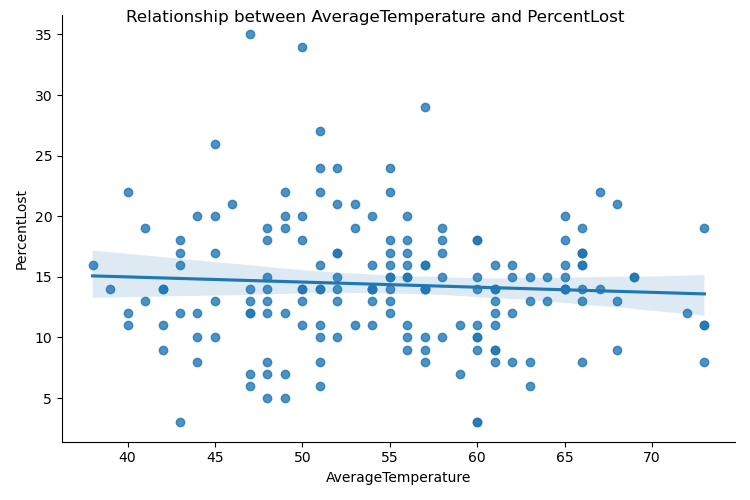
\includegraphics[width=0.8\textwidth,height=0.8\textheight]{../images/average_temperature_linearity.png}

}

\subcaption{\label{fig-average\_temperature}relationship between average
temperature and percentage loss}

\centering{

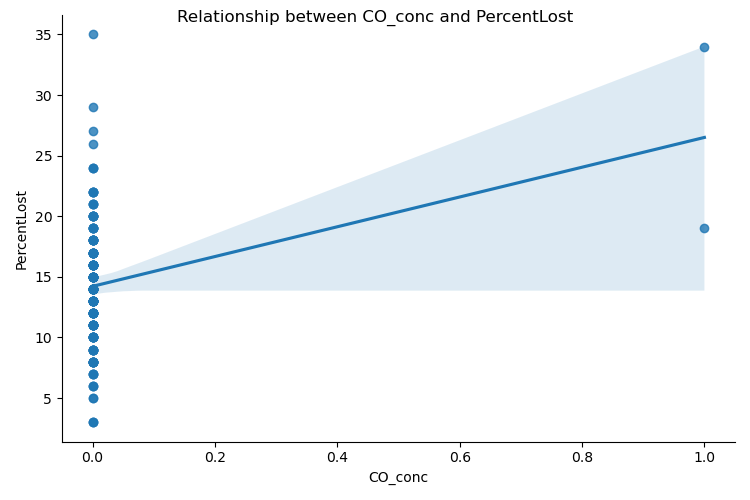
\includegraphics[width=0.8\textwidth,height=0.8\textheight]{../images/co_conc_linearity.png}

}

\subcaption{\label{fig-co\_conc}relationship between CO and percentage
loss}

\centering{

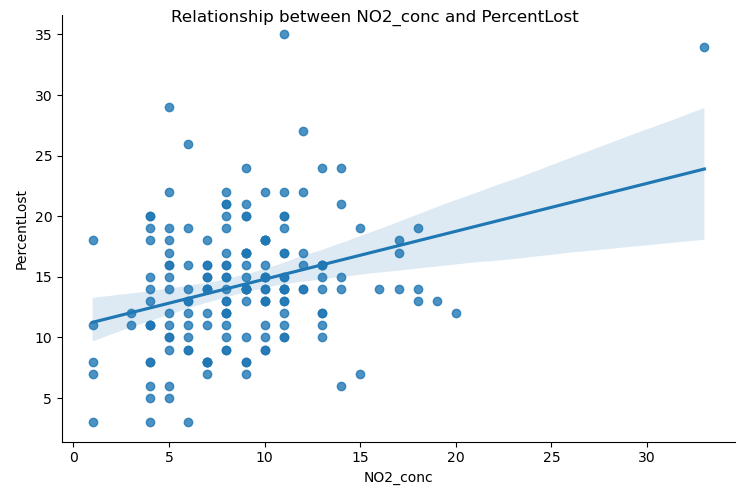
\includegraphics[width=0.8\textwidth,height=0.8\textheight]{../images/no2_conc_linearity.png}

}

\subcaption{\label{fig-no2\_conc}relationship between NO2 and percentage
loss}

\centering{

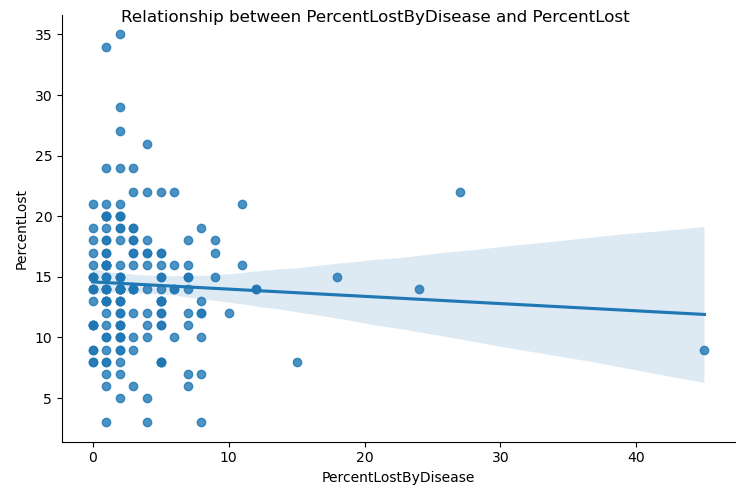
\includegraphics[width=0.8\textwidth,height=0.8\textheight]{../images/percent_lost_by_disease_linearity.png}

}

\subcaption{\label{fig-percent\_lost}relationship between percentage
loss by disease and percentage loss}

\centering{

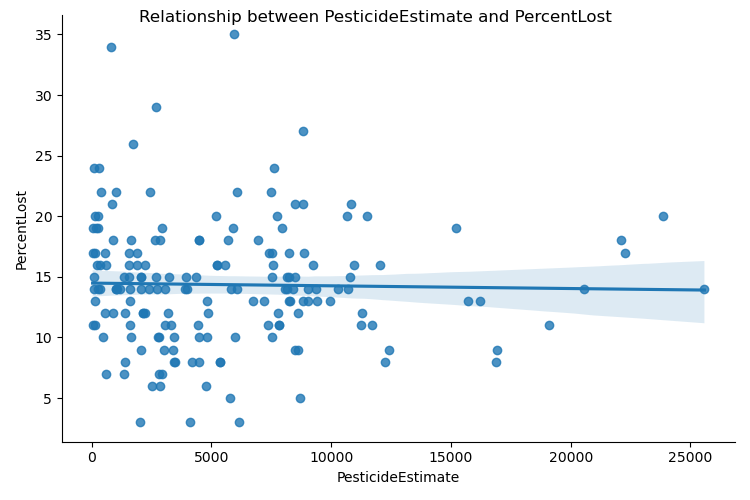
\includegraphics[width=0.8\textwidth,height=0.8\textheight]{../images/pesticide_estimate_linearity.png}

}

\subcaption{\label{fig-pesticide\_estimate\_linearity}relationship
between pesiticde estimate by disease and percentage loss}

\centering{

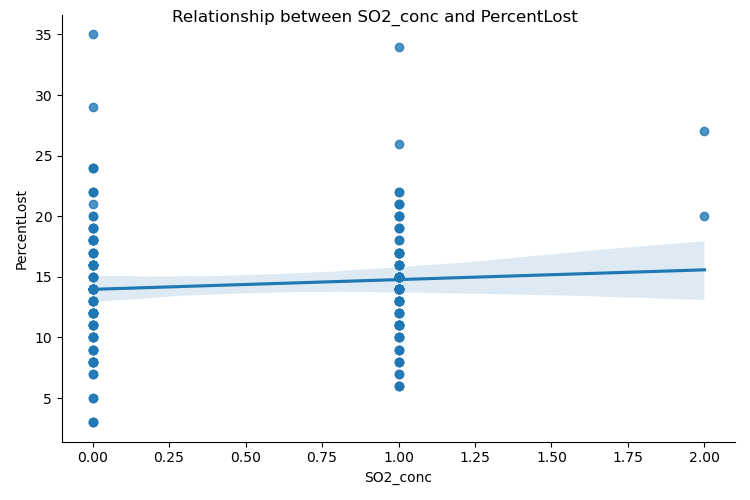
\includegraphics[width=0.8\textwidth,height=0.8\textheight]{../images/so2_conc_linearity.png}

}

\subcaption{\label{fig-so2\_conc}relationship between SO2 and percentage
loss}

}

\caption{\label{fig-linear\_relationships}linear relationships}

\end{figure}%

We initiated this exploration by investigating the linearity between our
key explanatory variables and the percentage loss of bee colonies. By
generating scatter plots accompanied by best-fit lines for each variable
against the percentage loss, we observed varying degrees of linearity.
From Figure~\ref{fig-linear_relationships}, notably, CO and NO2
concentrations demonstrated a clear positive trend, indicating a
potential association of increased pollutants with higher bee colony
losses. Conversely, SO2 concentrations exhibited a weaker and less
defined relationship, suggesting a potentially lesser or non-linear
impact on colony losses. Overall, the linearity assumption for linear
regression is only partially met.

\begin{longtable}[]{@{}lll@{}}

\caption{\label{tbl-vif}VIF summary}

\tabularnewline

\toprule\noalign{}
& Variable & VIF \\
\midrule\noalign{}
\endhead
\bottomrule\noalign{}
\endlastfoot
0 & AverageTemperature & 6.448131 \\
1 & CO\_conc & 1.080469 \\
2 & NO2\_conc & 5.968260 \\
3 & SO2\_conc & 2.182898 \\
4 & PercentLostByDisease & 1.601289 \\
5 & PesticideEstimate & 2.509423 \\

\end{longtable}

To address concerns of multicollinearity, which can inflate the variance
of linear regression coefficients and compromise the interpretability of
the model, we employed the Variance Inflation Factor (VIF). Our findings
are illustrated in Table~\ref{tbl-vif}, with all VIF scores remaining
under the commonly accepted threshold of 10, indicated that
multicollinearity was unlikely to be a significant issue in our dataset.
This reassurance allowed us to proceed without the need to eliminate or
merge variables to mitigate multicollinearity effects.

\begin{figure}

\centering{

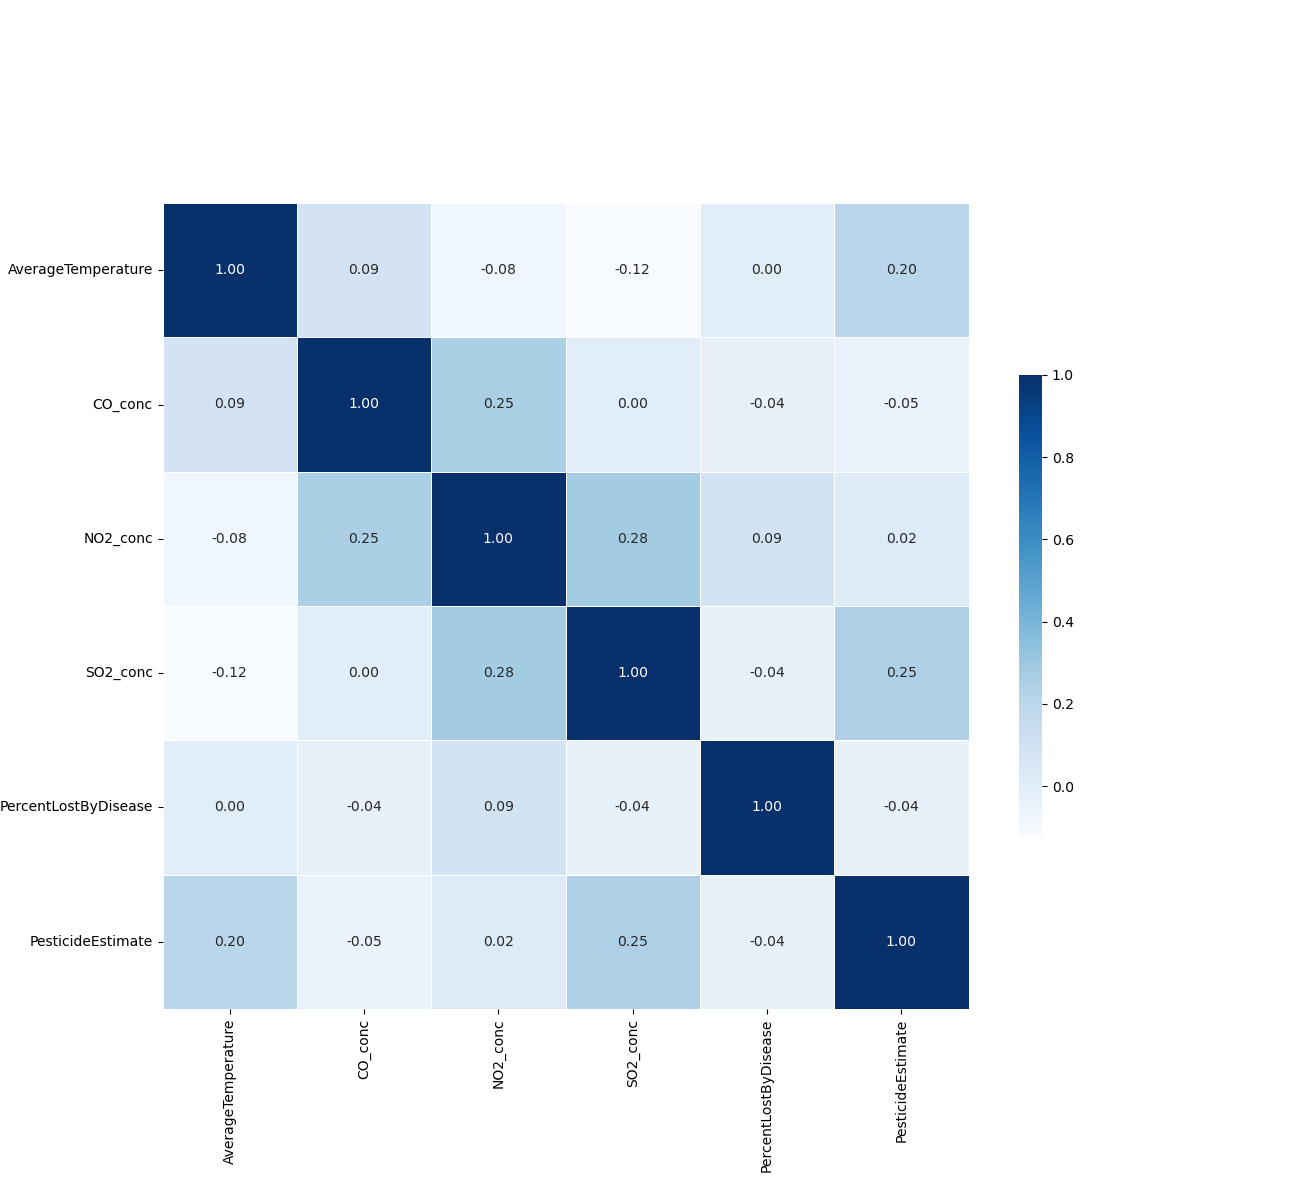
\includegraphics{../images/correlation_matrix.png}

}

\caption{\label{fig-correlation\_matrix}Correlation between each pair of
explanatory variables indicated by color intensity.}

\end{figure}%

Additionally, we scrutinized the correlations among our explanatory
variables to determine the necessity of including interaction terms in
our regression model. As shown in Figure~\ref{fig-correlation_matrix},
the resulting correlation matrix revealed the absence of strong
correlations between variables, as all the correlations are much smaller
than 0.5, thereby negating the need for interaction terms. This was a
crucial step in maintaining our model's simplicity and ensuring its
interpretability, adhering to the principle of Occam's razor in
statistical modeling.

Following our examination of linear relationships and correlations, we
opted for linear regression as our initial analytical strategy. This
choice was predicated on its simplicity, interpretability, and the
preliminary indication of linear associations between several variables
and the percentage loss of bee colonies. Linear regression allowed us to
quantify the strength and direction of these relationships under the
assumption that they hold a linear form, which is a common starting
point in statistical analysis for its straightforwardness and efficiency
in computation.

However, due to the absence of critical assumptions being fully met for
linear regression, it suggested a limited capacity to capture the
variability in bee colony losses. While carbon monoxide (CO) and
nitrogen dioxide (NO2) concentrations emerged as significant predictors,
the overall fit of the model highlighted the presence of potentially
unaccounted complex relationships or additional influential factors not
captured by our linear approach. In this case, investigation of
non-linear relationships between explanatory variables with bee colony
losses became crucial.

To explore the possibility of non-linear relationships influencing bee
colony losses, we turned to XGBoost, a decision-tree-based ensemble
machine learning algorithm known for its high performance and
flexibility. XGBoost is particularly adept at handling non-linear data,
making it an excellent candidate for our analysis. It can automatically
learn complex patterns through its ensemble of decision trees and is
capable of handling the interactions between features effectively, a
potential limitation in linear models. Additionally, XGBoost includes
regularization, which helps in preventing overfitting, a common concern
when modeling complex relationships.

In summary, our exploration through linear and non-linear models
underscores the challenges in modeling the factors affecting bee colony
losses. The limited success of both approaches points towards the need
for further investigation into other potential influencing factors,
better quality data, or more sophisticated modeling techniques to
capture the underlying dynamics more accurately. This journey through
linear to non-linear modeling illustrates the iterative nature of data
analysis, where initial findings often lead to new questions and
subsequent analytical explorations.

\section{Results}\label{results}

\subsection{Results from data
visualizations}\label{results-from-data-visualizations}

\begin{figure}

\centering{

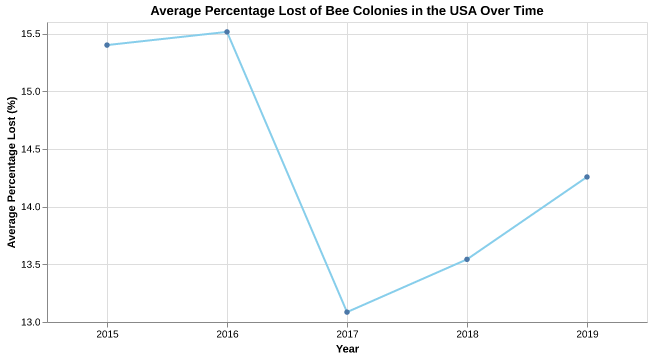
\includegraphics{../images/year_lost.png}

}

\caption{\label{fig-year\_lost}Average percentage loss of bees in the
USA from 2015 to 2019.}

\end{figure}%

Based on Figure~\ref{fig-year_lost}, we can observe that the average
percentage loss of bee colonies differs over the 5-year period. The
average percentage loss of bee colonies slightly increased from 2015 to
2016, then decreased from 15.5\% to about 13.1\% from 2016 to 2017.
However, this percentage loss continued to increase for 2018 and 2019.
The highest percentage loss occurred in 2016 (15.5\%).

\begin{figure}

\centering{

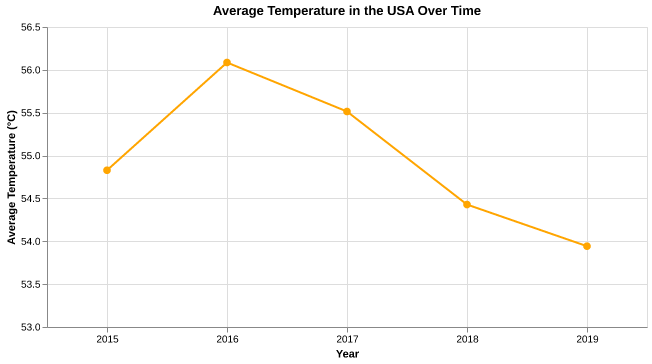
\includegraphics{../images/year_temperature.png}

}

\caption{\label{fig-year\_temp}Average temperature in the USA from 2015
to 2019.}

\end{figure}%

Regarding average temperature Figure~\ref{fig-year_temp}, it increased
from 54.8°C to 56.1°C from 2015 to 2016, reaching the highest
temperature among the 5 years, then decreased over the following three
years. Since 2016 had both the highest average temperature and the
highest average percentage loss for the USA, it may imply a potential
association between temperature and bee health.

\begin{figure}

\centering{

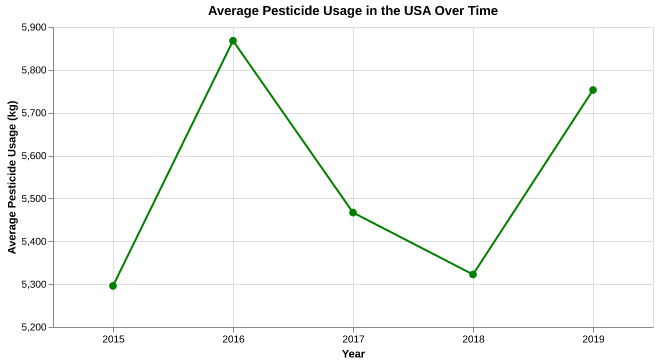
\includegraphics{../images/year_pesticide.png}

}

\caption{\label{fig-year\_pest}Average pesticide usage in the USA from
2015 to 2019.}

\end{figure}%

In terms of pesticide usage in the USA Figure~\ref{fig-year_pest}, the
amount increased from 5300 kg in 2015 to its peak usage, approximately
5890 kg in 2016. Subsequently, the usage decreased over time until 2018,
reaching about 5310 kg. The usage then increased to approximately 5750
kg in 2019. Since 2016 had both the highest pesticide usage and the
highest average percentage loss of bees for the USA, it suggests a
potential association between pesticide usage and bee health.

\begin{figure}

\centering{

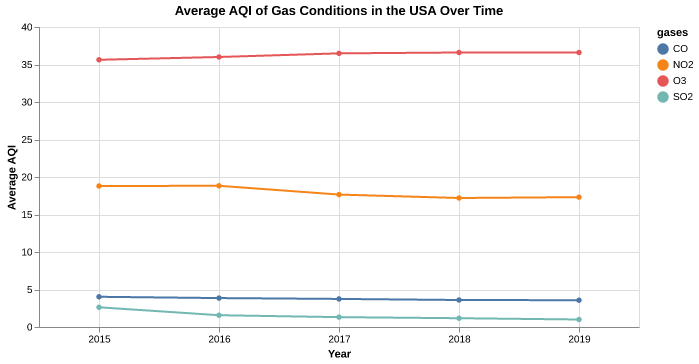
\includegraphics{../images/year_aqi.png}

}

\caption{\label{fig-year\_aqi}Average AQI of gas conditions in the USA
from 2015 to 2019.}

\end{figure}%

In terms of Average AQI Figure~\ref{fig-year_aqi}, all four gases do not
seem to change much between years in the USA. Since a higher AQI value
indicates greater levels of air pollution and greater health concerns
(Bishoi et al., 2009), O3 has the highest value of the Average AQI,
posing the highest risk of contributing to bee health among these four
gases, followed by NO2, CO, and SO2.

\subsection{Results from regression
models}\label{results-from-regression-models}

\begin{table}

\caption{\label{tbl-ols}Results of linear regression.}

\centering{

\begin{verbatim}
                     Results: Ordinary least squares
=========================================================================
Model:                 OLS                Adj. R-squared:       0.110    
Dependent Variable:    PercentLost        AIC:                  1058.9125
Date:                  2024-06-05 03:12   BIC:                  1087.3956
No. Observations:      175                Log-Likelihood:       -520.46  
Df Model:              8                  F-statistic:          3.679    
Df Residuals:          166                Prob (F-statistic):   0.000561 
R-squared:             0.151              Scale:                23.641   
-------------------------------------------------------------------------
                      Coef.   Std.Err.    t    P>|t|    [0.025    0.975] 
-------------------------------------------------------------------------
const                632.0818 547.6184  1.1542 0.2501 -449.1130 1713.2765
Year                  -0.3058   0.2712 -1.1274 0.2612   -0.8413    0.2297
AverageTemperature    -0.0553   0.0526 -1.0515 0.2946   -0.1591    0.0485
PercentLostByDisease  -0.0745   0.0748 -0.9962 0.3206   -0.2222    0.0732
CO_conc                8.9131   3.6597  2.4355 0.0159    1.6875   16.1387
NO2_conc               0.3263   0.1001  3.2612 0.0013    0.1288    0.5239
SO2_conc              -0.3515   0.8154 -0.4311 0.6670   -1.9614    1.2584
PesticideEstimate      0.0000   0.0001  0.0126 0.9899   -0.0002    0.0002
State_encoded         -0.0244   0.0420 -0.5812 0.5619   -0.1074    0.0586
-------------------------------------------------------------------------
Omnibus:                20.420         Durbin-Watson:            1.571   
Prob(Omnibus):          0.000          Jarque-Bera (JB):         29.597  
Skew:                   0.673          Prob(JB):                 0.000   
Kurtosis:               4.500          Condition No.:            11358072
=========================================================================
Notes:
[1] Standard Errors assume that the covariance matrix of the errors is
correctly specified.
[2] The condition number is large, 1.14e+07. This might indicate
that there are strong multicollinearity or other numerical
problems.
\end{verbatim}

}

\end{table}%

The linear regression results show that the model explains approximately
11\% of the variability in the percent loss of bee colonies, as
indicated by the adjusted R-squared value from Table~\ref{tbl-ols}.
Among the variables, carbon monoxide concentration (CO\_conc) and
nitrogen dioxide concentration (NO2\_conc) are statistically significant
at the 5\% level, suggesting a potential association with the percent
loss of bee colonies. The significance of these pollutants highlights
them as factors that could influence bee colony losses. However, the low
R-squared value suggests that the model does not fit the data very well,
meaning that there are other unaccounted factors or complex
relationships that influence the percent loss of bee colonies. The
variables for year, average temperature, ozone concentration (O3\_conc),
sulfur dioxide concentration (SO2\_conc), and state encoded as numeric
values were not found to be significant predictors in this model.

Upon applying XGBoost to our data, we aimed to uncover non-linear
patterns that linear regression may have missed. The model's predictive
performance, as measured by R-squared, was approximately 0.0667,
indicating only a slight improvement in capturing the variability of bee
colony losses compared to the linear model. This outcome suggested that
while non-linear patterns might exist, they are either too intricate or
too weakly associated with the data we have, or that other unaccounted
factors play a more significant role than those we included in our
model.

\begin{figure}

\centering{

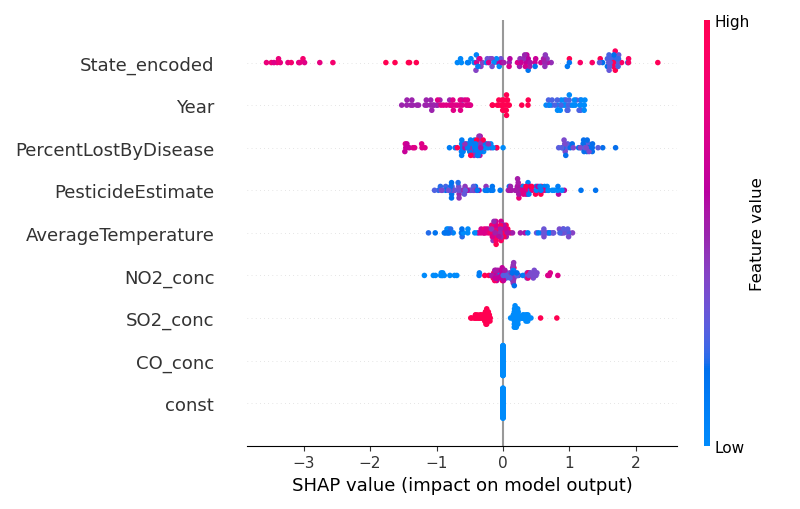
\includegraphics{../images/shap_train.png}

}

\caption{\label{fig-shap\_train}Distribution of SHAP value for each
predictors in the XGBoost model.}

\end{figure}%

\begin{figure}

\centering{

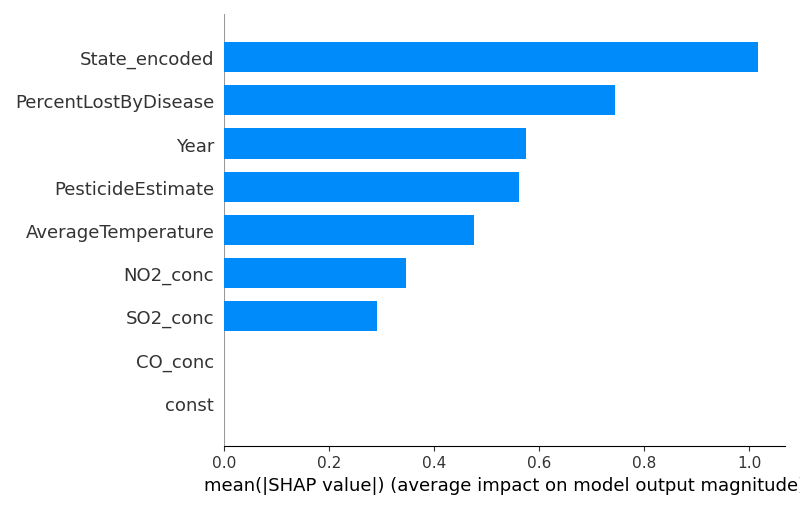
\includegraphics{../images/shap_overall.png}

}

\caption{\label{fig-shap\_overall}Feature Importance Plot for the
XGBoost model.}

\end{figure}%

The SHAP (SHapley Additive exPlanations) analysis provided further
insights into the influence of individual features on the XGBoost
model's predictions, and the results are presented in
Figure~\ref{fig-shap_train}. The significant impact of features such as
State and Year, as indicated by their SHAP values in
Figure~\ref{fig-shap_overall}, hinted at the complex interplay of
temporal and geographical factors with bee colony health. However, given
the overall low performance of the XGBoost model with an adjusted
R-squared value of 0.0667, the XGBoost model has limited predictive
power and explains only about 6.67\% of the variance in the percent loss
of bee colonies, and the findings must be interpreted with caution. They
suggest that while certain variables show a stronger influence, the
model's capacity to accurately predict bee colony losses remains
limited, underlining the complexity of the issue and the possibility of
missing crucial explanatory variables or facing data quality issues.

\section{Discussion}\label{discussion}

In examining our findings, several limitations emerge that warrant
consideration. Firstly, the utilization of yearly temperature data,
averaged across all months, may obscure the nuances of temperature
fluctuations throughout the year, potentially hindering our ability to
discern associations between temperature and other factors. Analyzing
monthly temperature data would offer a more nuanced understanding of
seasonal temperature variations, thus enriching our analysis.
Additionally, variations in colony numbers by quarter, influenced by
factors such as summer heat and natural bee biological cycles, may
introduce complexities in interpreting colony trends. Moreover, the
cyclical nature of parasite infestations, particularly in wintering
states, underscores the importance of long-term monitoring to discern
recurring patterns and inform proactive measures to safeguard bee
health. Disparities in colony numbers between states further complicate
analysis, influenced by factors like bee species diversity, habitat
preferences, and unique environmental conditions. Methodologically,
refining detection methods for colony numbers and pesticide usage is
imperative, given the inherent biases introduced by larger states with
more colonies and higher pesticide usage rates. Overall, the process of
averaging to obtain yearly data results in a lack of specific changing
patterns of these factors. Consequently, drawing conclusive conclusions
based on the visualizations and regression models we built becomes
challenging.

\section{Future Directions}\label{future-directions}

Moving forward, several avenues for future research present themselves.
A more granular analysis of factors such as temperature and pesticide
usage using monthly data would yield insights into their fluctuations
and impacts on bee colonies, aligning with previous research documenting
seasonal colony loss rates (Kulhanek et al., 2017). Investigating
seasonal variations in colony numbers across states can elucidate the
interplay between environmental factors and bee biology, guiding
targeted management strategies. Long-term monitoring of parasite trends
in wintering states is essential to identify recurring patterns and
develop proactive measures to mitigate their impact on bee health.
Further exploration of state-specific factors contributing to
disparities in colony numbers, such as bee species composition and
habitat characteristics, promises to deepen our understanding of
regional variations in beekeeping practices and pesticide usage.
Methodological refinement, including the development of more
sophisticated techniques to adjust for geographical differences in
colony numbers and pesticide usage, will enhance the accuracy and
reliability of data analysis, facilitating more robust conclusions and
informed decision-making (Kulhanek et al., 2017).

\section{Data Concerns and Relational
vs.~Non-Relational}\label{data-concerns-and-relational-vs.-non-relational}

When contemplating the long-term maintenance of our project data,
several critical concerns emerge, particularly in the context of our
investigation into the intricate relationships affecting honey bee
populations and ecosystem sustainability.

\subsection{A. Concerns about long-term data
storage}\label{a.-concerns-about-long-term-data-storage}

As we delve into the analysis of factors impacting honey bee
populations, one of our foremost concerns lies in ensuring the
durability and accessibility of our data over time. Given the evolving
landscape of data storage technologies, there is a risk of data formats
becoming obsolete, potentially hindering our ability to retrieve or
utilize historical data. Furthermore, the accumulation of vast amounts
of data throughout the project's duration presents challenges in terms
of storage capacity and organization. It is imperative for us to
implement robust data management strategies to adapt to evolving
technologies and maintain the integrity and accessibility of our data
for future research endeavors.

\subsection{B. Preserving data
provenance}\label{b.-preserving-data-provenance}

The preservation of data provenance is another crucial aspect of our
long-term data maintenance strategy. As we collect and analyze data from
various sources, documenting the origin, processing steps, and any
transformations applied to the data is essential for ensuring
transparency, reproducibility, and accountability. By meticulously
documenting data provenance throughout the project lifecycle, we can
provide future researchers with the necessary context to validate and
replicate our findings, thereby contributing to the integrity and
reliability of scientific research in the field.

\subsection{C. Advantages of using a
database}\label{c.-advantages-of-using-a-database}

Given the unique parameters of our project, there are instances where
utilizing a database would offer distinct advantages over managing data
through a series of individual files. Specifically, a database becomes
advantageous when dealing with large volumes of interconnected data,
such as the multitude of variables influencing honey bee populations and
ecosystem dynamics. By leveraging a database, we can benefit from
features such as structured data management, scalability, efficient
query performance, and robust data integrity mechanisms. Additionally,
databases provide a platform for implementing advanced analytical
techniques and facilitating collaborative research efforts, making them
particularly well-suited for projects with complex data requirements and
analytical objectives.

When considering the advantages of using a database for our project,
it's essential to delve into the distinction between relational and
non-relational databases, and how each may suit our specific needs.

Relational databases, characterized by their structured approach to data
management using tables with predefined relationships between them,
offer several advantages for our project. For example, we can organize
our data into tables representing different aspects of honey bee
populations, such as colony health, environmental factors, and pesticide
usage. By establishing relationships between these tables, we can
efficiently query and analyze interconnected data, enabling us to
uncover complex patterns and relationships influencing honey bee
populations.

One concrete example of when a relational database would be advantageous
is in managing data on honey bee colony health and pesticide usage. We
can create separate tables for colony health metrics and pesticide
application data, linked by common identifiers such as geographic
location or time period. This relational structure allows us to perform
sophisticated analyses, such as identifying correlations between
specific pesticides and changes in colony health over time.

On the other hand, non-relational databases, also known as NoSQL
databases, offer flexibility and scalability for managing unstructured
or semi-structured data. While relational databases excel in managing
structured data with predefined schemas, non-relational databases are
better suited for handling diverse data types, such as sensor data or
social media feeds, without rigid schema requirements.

In our project, a non-relational database may be advantageous when
dealing with unstructured or semi-structured data sources, such as
climate sensor data or social media mentions of honey bee populations.
For example, we could use a document-oriented database to store and
analyze textual data from social media platforms, allowing us to
identify public perceptions or concerns about honey bee health and
correlate them with environmental factors.

In summary, the choice between using a relational or non-relational
database depends on the nature of the data and the specific requirements
of our project. Relational databases offer structured data management
and predefined relationships, making them suitable for managing
interconnected data on honey bee populations and ecosystem dynamics.
Non-relational databases, on the other hand, provide flexibility and
scalability for handling diverse data types, making them advantageous
for managing unstructured or semi-structured data sources. In our case,
since we are more interested in the relationships between different
factors contributing to the loss of bees in the USA than in textual data
from social media, etc., we believe a relational database will be more
suitable. Additionally, the types of data we will be collecting are easy
to handle in relational databases.



\end{document}
